%
%  untitled
%
%  Created by António Sousa on 2010-11-03.
%  Copyright (c) 2010 __MyCompanyName__. All rights reserved.
%
\documentclass[a4paper,12pt,portugues]{article}

% Use utf-8 encoding for foreign characters
\usepackage[utf8]{inputenc}
\usepackage[T1]{fontenc}
\usepackage[portuges]{babel}

% Setup for fullpage use
%\usepackage{fullpage}

% Uncomment some of the following if you use the features
%
% Running Headers and footers
%\usepackage{fancyhdr}

% Multipart figures
%\usepackage{subfigure}

% More symbols
%\usepackage{amsmath}
%\usepackage{amssymb}
%\usepackage{latexsym}

% Surround parts of graphics with box
\usepackage{boxedminipage}

% Package for including code in the document
\usepackage{listings}


% This is now the recommended way for checking for PDFLaTeX:
\usepackage{ifpdf}

\ifpdf
\usepackage[pdftex]{graphicx}
\else
\usepackage{graphicx}
\fi

\usepackage{rotating}



\title{Eurotux Virtual Appliance - ETVA\\
Relatório Técnico-Científico}
\author{Eurotux Informática, SA}

\date{2010-11-03}

\begin{document}

\ifpdf
\DeclareGraphicsExtensions{.pdf, .jpg, .tif}
\else
\DeclareGraphicsExtensions{.eps, .jpg}
\fi

\maketitle


% \begin{abstract}
% \end{abstract}

\section{Sumário executivo} % (fold)
\label{sec:sumario_executivo}

% Sumário executivo das actividades do projecto e dos resultados alcançados
% Nesta secção inclua uma descrição sucinta dos objectivos do projecto, do
% trabalho realizado desde o início do projecto e dos principais resultados
% alcançados até ao período de reporte.


O projecto Eurotux Virtual Appliance (ETVA), tem como objectivo o
desenvolvimento de uma plataforma computacional com o formato de appliance e
potenciadora da adopção de programas e ferramentas open-source em ambiente
empresarial.

Com este projecto a Eurotux pretende desenvolver um novo produto que se
acredita ser inovador no mercado e que permitirá a custos controlados oferecer
a um universo de micro, pequenas e médias empresas (que são a maioria das
empresas existentes em Portugal) o acesso a soluções tecnológicas apenas
acessíveis a organizações de maiores dimensões e com equipas de TI dedicadas.

Tendo consciência da dimensão das empresas e das dificuldades que estas
poderão ter na aquisição de uma solução totalmente redundante, a Eurotux
pretende disponibilizar ao mercado a ETVA em duas versões. A versão SMB será o
mais compacta possível e será redundante apenas nos componentes fundamentais
de forma a reduzir os custos de aquisição e manutenção. Por seu lado a versão
enterprise será totalmente redundante, oferecendo garantias de desempenho e
confiabilidade muito superiores mas que será indicada para empresas já com
alguma dimensão.

O projecto foi dividido em seis actividades de desenvolvimento e uma adicional
de gestão do projecto. Destas actividades quatro estão relacionadas com o
desenvolvimento do produto sendo as restantes duas relacionadas com a
divulgação dos resultados obtidos e outra com o controlo de qualidade e gestão
de processos associados à ETVA.

Numa primeira fase de investigação procurou-se quer na indústria quer na
comunidade académica trabalhos relacionados com o que pretendíamos para a
ETVA, permitindo-nos concluir que apesar de existirem algumas abordagens à
gestão centralizada e uniformizada de infraestruturas nenhuma delas possuía o
grau de integração que almejavamos com ETVA.

Assim sendo passou-se a uma fase de planeamento em que se procurou encontrar
soluções para dois problemas distintos. O primeiro qual a plataforma de
virtualização a adoptar e o segundo qual a interface gráfica e API
(Webservices) a desenvolver para fazer a integração entre a consola de gestão
e os serviços por ela geridos.

Para o primeiro problema a solução não foi fácil de encontrar, pois sendo uma
tecnologia relativamente recente e em franco desenvolvimento, a principal
preocupação foi em adoptar uma que desse garantias de continuidade no futuro.
Esta escolha, teve impacto no projecto, tendo sido responsável por alguns dos
atrasos verificados. Achámos que conseguimos uma solução de compromisso ao
adoptarmos uma solução de middleware que à partida permitirá não ficarmos
presos a uma única solução de virtualização.

Após este trabalho inicial os trabalhos passaram a decorrer em bom ritmo tendo
sido cumpridos os objectivos que nos tinhamos proposto, tendo neste momento
dois protótipos demonstráveis. Um para PME's conistindo numa appliance que foi
seleccionada no decurso na tarefa 4 e o outro para médias empresas com parques
computacionais maiores e cujo protótipo está disponível nos equipamentos
adquiridos por este projecto.

Relativamente à tarefa de migração dos produtos Eurotux para a ETVA, face à
oferta de mercado, optámos por remover a integração do produto "Eurotux
Virtual Hotspot" e passar a integrar um novo denominado de "Eurotux Voip
Server". Este, permite dotar a empresa de uma solução de telefonia sobre IP de
forma a minimizar custos e maximizar a eficiência de processos.

% section sumário_executivo (end)

\section{Execução do projecto} % (fold)
\label{sec:execucao_do_projecto}
% 2- Diagrama de Gantt comparando o trabalho previsto na candidatura com o
% realizado

O trabalho realizado previsto e realizado no âmbito do projecto da Eurotux
Virtual Appliance está descito na Figura~\ref{fig:gantt}. Nesta figura e para
cada tarefa apresentam-se duas linhas, uma em tons de cinzento com a duração
prevista em projecto para cada uma das tarefas e outra em tons de verde ou
laranja para com a duração efectivadas tarefas. Durações em laranja estão
relacionadas com actividades que não foram inteiramente realizadas ou que se
decidiu substituir por outras que foram consideradas mais relevantes para o
projecto.

O projecto da Eurotux Virtual Appliance, está, tal como pode ser observado na
Figura~\ref{fig:gantt} está dividido em 7 actividades, descritas nos parágrafos seguintes.

Na actividade 1 - Arquitectura de Serviços da ETVA, forma previstas 4 tarefas,
duas iniciais de levantamento do estado da arte e definição da arquitectura de
serviços a utilizar e implementar, que decorreram nos prazos previstos. Das
restantes duas tarefas: \emph{i} implementação da arquitectura SOA e;
\emph{ii} serviços na Eurotux Virtual Appliance e implementação do serviço de
directoria, a primeira revelou-se mais complicada do que o inicialmente
previsto, devido também à necessidade sentida de não ficar preso a um único
sistema de virtualização, tendo os trabalhos desta sido prolongados por mais
oito meses do que inicialmente previsto. Relativamente à segunda tarefa e
apesar de ter sido planeada a arquitectura do serviço de directoria e dado que
a sua relevância é primordial apenas quando o serviço estiver no mercado,
optou-se por não a implementar nesta fase, o que está descrito na
Figura~\ref{fig:gantt} com os milestones marcados a vermelho e o trabalho
executado a laranja.

\begin{figure}[htbp]
	\centering
	\begin{turn}{90}
		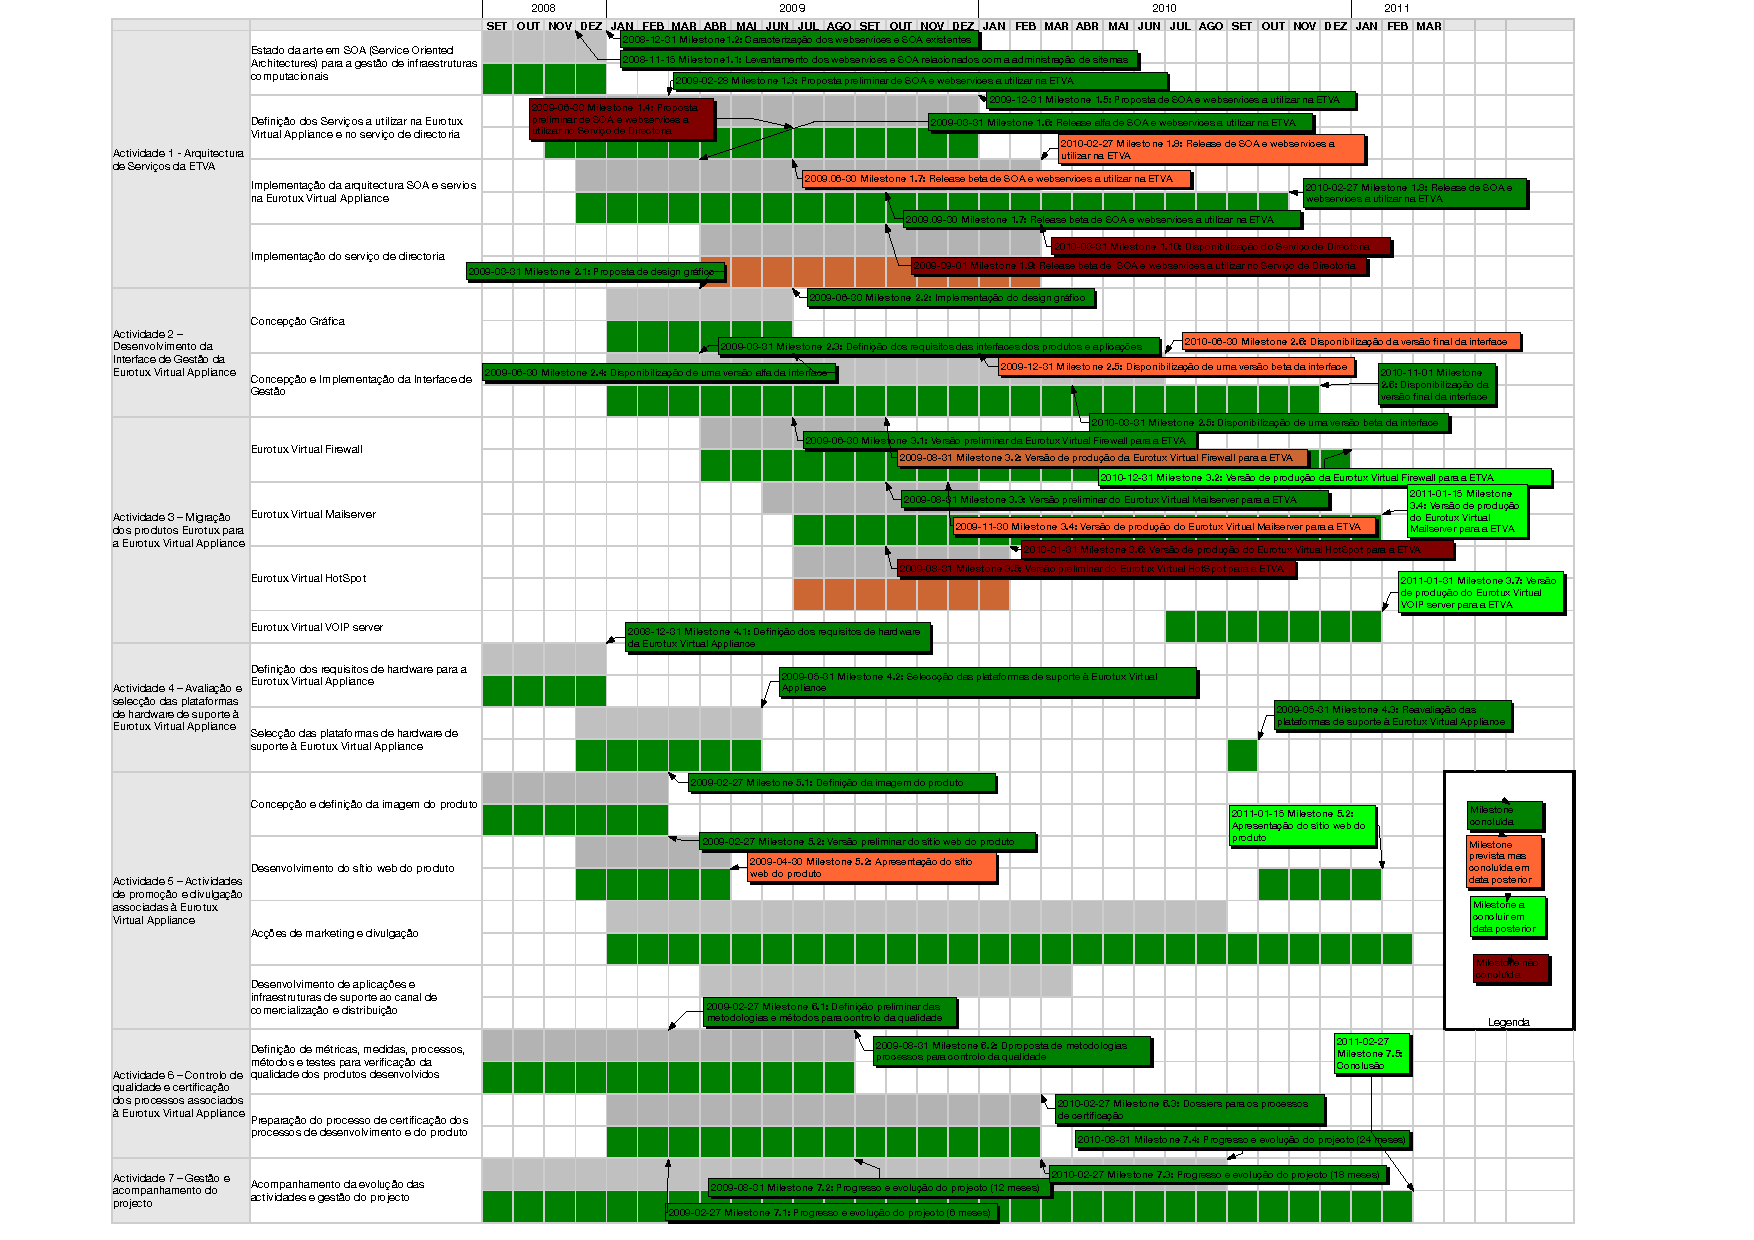
\includegraphics[scale=.65]{gantt}
	\end{turn}
	\caption{Gantt do projecto ETVA}
	\label{fig:gantt}
\end{figure}

Na Actividade 2 – Desenvolvimento da Interface de Gestão da Eurotux Virtual
Appliance, foram previstas duas tarefas: \emph{i} Concepção Gráfica e;
\emph{ii} Concepção e Implementação da Interface de Gestão. A primeira tarefa
decorreu como previsto, tendo sido definida uma arquitectura básica para
interface com o utilizador e definido o modelo de implementação utilizando o
padrão MVC~\cite{mvc}. Na segunda tarefa, e resultante dos atrasos verificadas
na actividade 1, o segundo e terceiro milestones desta actividade foram
diferidos de três e cinco meses respectivamente.

Na Actividade 3 – Migração dos produtos Eurotux para a Eurotux Virtual
Appliance, o plano inicial para a sua execução começou a ser executado tal
como planeado, mas teve que ser revisto e os prazos de conclusão dilatados,
devido aos atrasos verificados nas Actividades 1 e 2. Em relação às duas
primeiras tarefas elas foram iniciadas como previsto e a versão preliminar
ficou concluída nos instantes previstos, mas as versões finais só estão
previstas uma para o final do ano de 2010 e a outra para o mês de Janeiro de
2011. Relativamente à terceira tarefa desta actividade, o Eurotux Virtual
HotSpot, foi considerado pela equipa de desenvolvimento e pela própria empresa
um produto que não seria essencial e optou-se por incluir o Eurotux Virtual
VOIP server. Este produto não estava previsto mas do ponto de vista da Eurotux
tem muito maior potencial para captar a atenção dos potenciais clientes.
Espera-se ter este produto integrado na ETVA no final do mês de Janeiro de
2011.

A Actividade 4 – Avaliação e selecção das plataformas de hardware de suporte à
Eurotux Virtual Appliance, decorreu conforme o planeado tendo sido cumpridos
os timings previstos, tendo resultado deste trabalho a definição de dois tipos
de plataformas de suporte à ETVA. Devido à constante evolução das plataformas
computacionais, nesta actividade foi adicionado um milestone adicional
correspondente a actividades realizadas durante o mês de Setembro de 2011 de
que resultou a revisão das plataformas escolhidas para o mercado das pequenas
e micro-empresas.

Relativamente à Actividade 5 – Actividades de promoção e divulgação associadas
à Eurotux Virtual Appliance, os primeiros objectivos de construção de um sítio
web para o produto e a construção de uma imagem de marca foram realizados no
início do projecto para marcar presença do mesmo na web. As restantes
actividades de promoção não foram ainda realizadas estando previsto para o mês
de Janeiro de 2011 a apresentação do sítio web do produto completamente
reformulado e preparado para o lançamento do produto. Ainda durante os dois
primeiros meses de 2011 está prevista a participação em eventos internacionais
com o intuito de promover a ETVA.

Relativamente à Actividade 6 – Controlo de qualidade e certificação dos
processos associados à Eurotux Virtual Appliance, esta foi especialmente
importante pois revolucionou algumas das formas de trabalhar da Eurotux,
nomeadamente na forma como é feita a gestão e acompanhamento de projectos.
Numa primeira fase, definiu métodos e mecanismos para manter actualizada a
documentação e evolução dos trabalhos referentes à ETVA. Como resultado do
trabalho levado a cabo por esta actividade a Eurotux definiu como estratégia
implementar um projecto de certificação de processos ISO9001 e de IDI (NP
4457).


A Actividade 7 – Gestão e acompanhamento do projecto, tal como previsto
acompanhou de perto os trabalhos realizados, tendo notificado a partir dos 12
meses de projecto que poderiam existir alguns atrasos no calendário previsto.
Para acompanhar extensão da duração do projecto, esta actividade foi estendida
por mais 6 meses e adicionado um novo milestone associado à conclusão do
projecto.

 % section execução_do_projecto (end)

\section{Resultados obtidos} % (fold)
\label{sec:resultados_obtidos}

% 3- Apresentação dos resultados alcançados por tarefa, justificando
% eventuais desvios face ao previsto em candidatura Se aplicável, explicite
% alterações aos objectivos críticos definidos, por não terem sido atingidos
% e/ou por os desenvolvimentos terem gerado novos resultados intermédios,
% justificando o impacto no projecto.


\subsection{Actividade 1 - Arquitectura de Serviços da Eurotux Virtual Appliance} % (fold)

Nesta actividade procura identificar-se quais os serviços e tecnologias
existentes no mercado que são importantes para o desenvolvimento do núcleo da
ETVA e que será sem qualquer sombra de dúvida a nível tecnológico o factor
distintivo desta.


\paragraph{Estado da arte em SOA (Service Oriented Architectures) para a gestão de infraestruturas computacionais} % (fold)

Nesta tarefa fez-se uma pesquisa sobre a existência de serviços ou interfaces/
definição de interfaces de gestão para parques computacionais. De todo este
trabalho de pesquisa ficou evidente que não existiam definidos este tipo de
serviços, pelo que o trabalho a realizar na tarefa seguinte teria que passar
pela definição de todas as interfaces para permitir a gestão centralizada de
todas as appliances a disponibilizar na ETVA.

\paragraph{Definição dos Serviços a utilizar na Eurotux Virtual Appliance e no serviço de directoria} % (fold)

Nesta tarefa foram definidos os requisitos e api a implementar como webservices na ETVA e appliances de forma a permitir a gestão dessas mesmas appliances a partir da consola de gestão da ETVA.



\paragraph{Implementação da arquitectura SOA e serviços na Eurotux Virtual Appliance} % (fold)

Nesta tarefa em que se tiveram de fazer escolhas tecnológicas com impacto na
execução do projecto e evolução futura da ETVA verificaram-se alguns atrasos
devidos à dificuldade de escolha da plataforma de virtualização a utilizar.
Durante esta fase do projecto existiram desenvolvimentos significativos nas
plataformas de virtualização, não sendo trivial a adopção de uma em
detrimentos de outras, de forma que foi feito um trabalho significativo de
forma a poder suportar diferentes plataformas de virtualização na ETVA.

O esforço dispendido nesta fase do projecto em suportar diferentes plataformas
de virtualização, julga-se justificado pela criação de um nível de abstracção
que permite facilmente alterar a plataforma de virtualização sem que isso
tenha impacto na interface de gestão e ciclo de vida das appliances.

\paragraph{Implementação do serviço de directoria} % (fold)

O serviço de directoria está pensado para funcionar como plataforma de
disponibilização de actualizações e de novas appliances para a ETVA, mas ainda
não foi implementado dado ser essencial numa fase posterior em que o produto
esteja já no mercado.

\subsubsection{Actividade 2 – Desenvolvimento da Interface de Gestão da
Eurotux Virtual Appliance} % (fold)

Esta actividade tem como objectivo definir e implementar uma interface de gestão unificada para as várias appliances a disponibilizar na ETVA.


\paragraph{Concepção Gráfica} % (fold)

Nesta tarefa definiram-se os requisitos da interface de gestão da ETVA, assim
como o desenho da interface a disponibilizar, quer seja para gerir o ciclo de
vida de uma appliance quer seja para a gestão destas.

\paragraph{Concepção e Implementação da Interface de Gestão} % (fold)

Esta tarefa implementou a interface definida na tarefa anterior utilizando
paro o efeito um toolkit de programação web com suporte a MVC~\cite{mvc}.
Os objectivos desta tarefa foram totalmente atingidos, tendo no entanto a
sua execução sofrido alguns atrasos devido ao atraso verificado na Actividade 1.


\subsubsection{Actividade 3 – Migração dos produtos Eurotux para a Eurotux Virtual Appliance} % (fold)

Esta tarefa tem como principal objectivo fazer uma prova de conceito que a
arquitectura desenvolvida no ETVA é genérica o suficiente para permitir o
deployment dos produtos Eurotux, assim como outros produtos. Nesta tarefa,
decidiu-se não implementar o Eurotux Virtual HotSpot e substituílo pelo
Eurotux Virtual VOIP server, que na conjuntura actual do mercado acreditamos
ter um potencial de aceitação muito superior

\paragraph{Eurotux Virtual Firewall} 

Este produto está completamente implementado na ETVA, estando pronto a entrar
em fase de testes quer internamente na Eurotux quer em clientes seleccionados.

\paragraph{Eurotux Virtual Mailserver}

O Virtual Mailserver teve alguns atrasos no desenvolvimento. Fruto dos
conhecimentos da Eurotux não só na gestão de email mas também de filtragem de
SPAM foi desenhada uma nova arquitectura para este serviço que terá como
resultado a completa integração com o serviço de filtragem de email da
Eurotux, resultando daqui um valor acrescentado para os clientes. Esta
appliance deve estar completamente desenvolvida e integrada na ETVA no início
de 2011.

\paragraph{Eurotux Virtual HotSpot}

Apesar de não estar fora dos planos da Eurotux o desenvolvimento desta
appliance, foi considerado mais relevante suportar telefonia IP na ETVA, razão
pela qual se substituiu esta tarefa pela Eurotux Virtual VOIP server.

\paragraph{Eurotux Virtual VOIP server}

Esta appliance tem como objectivo fazer a transição para VOIP das comunicações
telefónicas, promovendo a unificação das redes de voz e dados. Utilizando esta
appliance será fácil ás organizações aderirem ao VOIP permitindo além disso a
integração com outros serviços da organização disponibilizados pela ETVA.


\subsubsection{Actividade 4 – Avaliação e selecção das plataformas de hardware
de suporte à Eurotux Virtual Appliance}

Esta tarefa teve como objectivo e dados os requisitos funcionais da ETVA
definir a/as plataformas de hardware que melhor se adequam aos objectivos da
ETVA, nomeadamente ter uma versão entry level para pequenas organizações e uma
entreprise para organizações que estejam em fase de expansão e ou consolidação
das suas plataformas computacionais.

\paragraph{Definição dos requisitos de hardware para a Eurotux Virtual
Appliance}

Esta taerfa decorreu como o planeado e definindo quais os requisitos do hardware que permitiriam atingir os objectivos propostos na ETVA.

\paragraph{Selecção das plataformas de hardware de suporte à Eurotux Virtual Appliance}

Nesta tarefa foram seleccionadas plataformas para cada uma das versões a
disponibilizar, sendo que essa mesma escolha foi revista numa fase posterior
do projecto para garantir que as plataformas escolhidas para suportar a ETVA
estão actualizadas tecnologicamente.


\subsubsection{Actividade 5 – Actividades de promoção e divulgação associadas à Eurotux Virtual Appliance}


Esta actividade tem como principal objectivo dar a conhecer e promover o
trabalho realizado no âmbito da ETVA. A primeira tarefa tem como objectivo
construir uma imagem para o produto ETVA e a segunda garantir a sua divulgação
na internet com a construção do sítio web do produto.

\paragraph{Concepção e definição da imagem do produto}

Esta tarefa decorreu dentro dentro dos timings previstos resultando na
concepção de um logotipo (Figura~\ref{fig:logo}) para o produto e um sítio web alinhado com a imagem
da Eurotux (Figura~\ref{fig:site}).

\begin{figure}[htbp]
	\centering
	%\begin{turn}{90}
		
\includegraphics[scale=.65]{logo}
	%\end{turn}
	\caption{Logotipo da ETVA}
	\label{fig:logo}
\end{figure}

\begin{figure}[htbp]
	\centering
		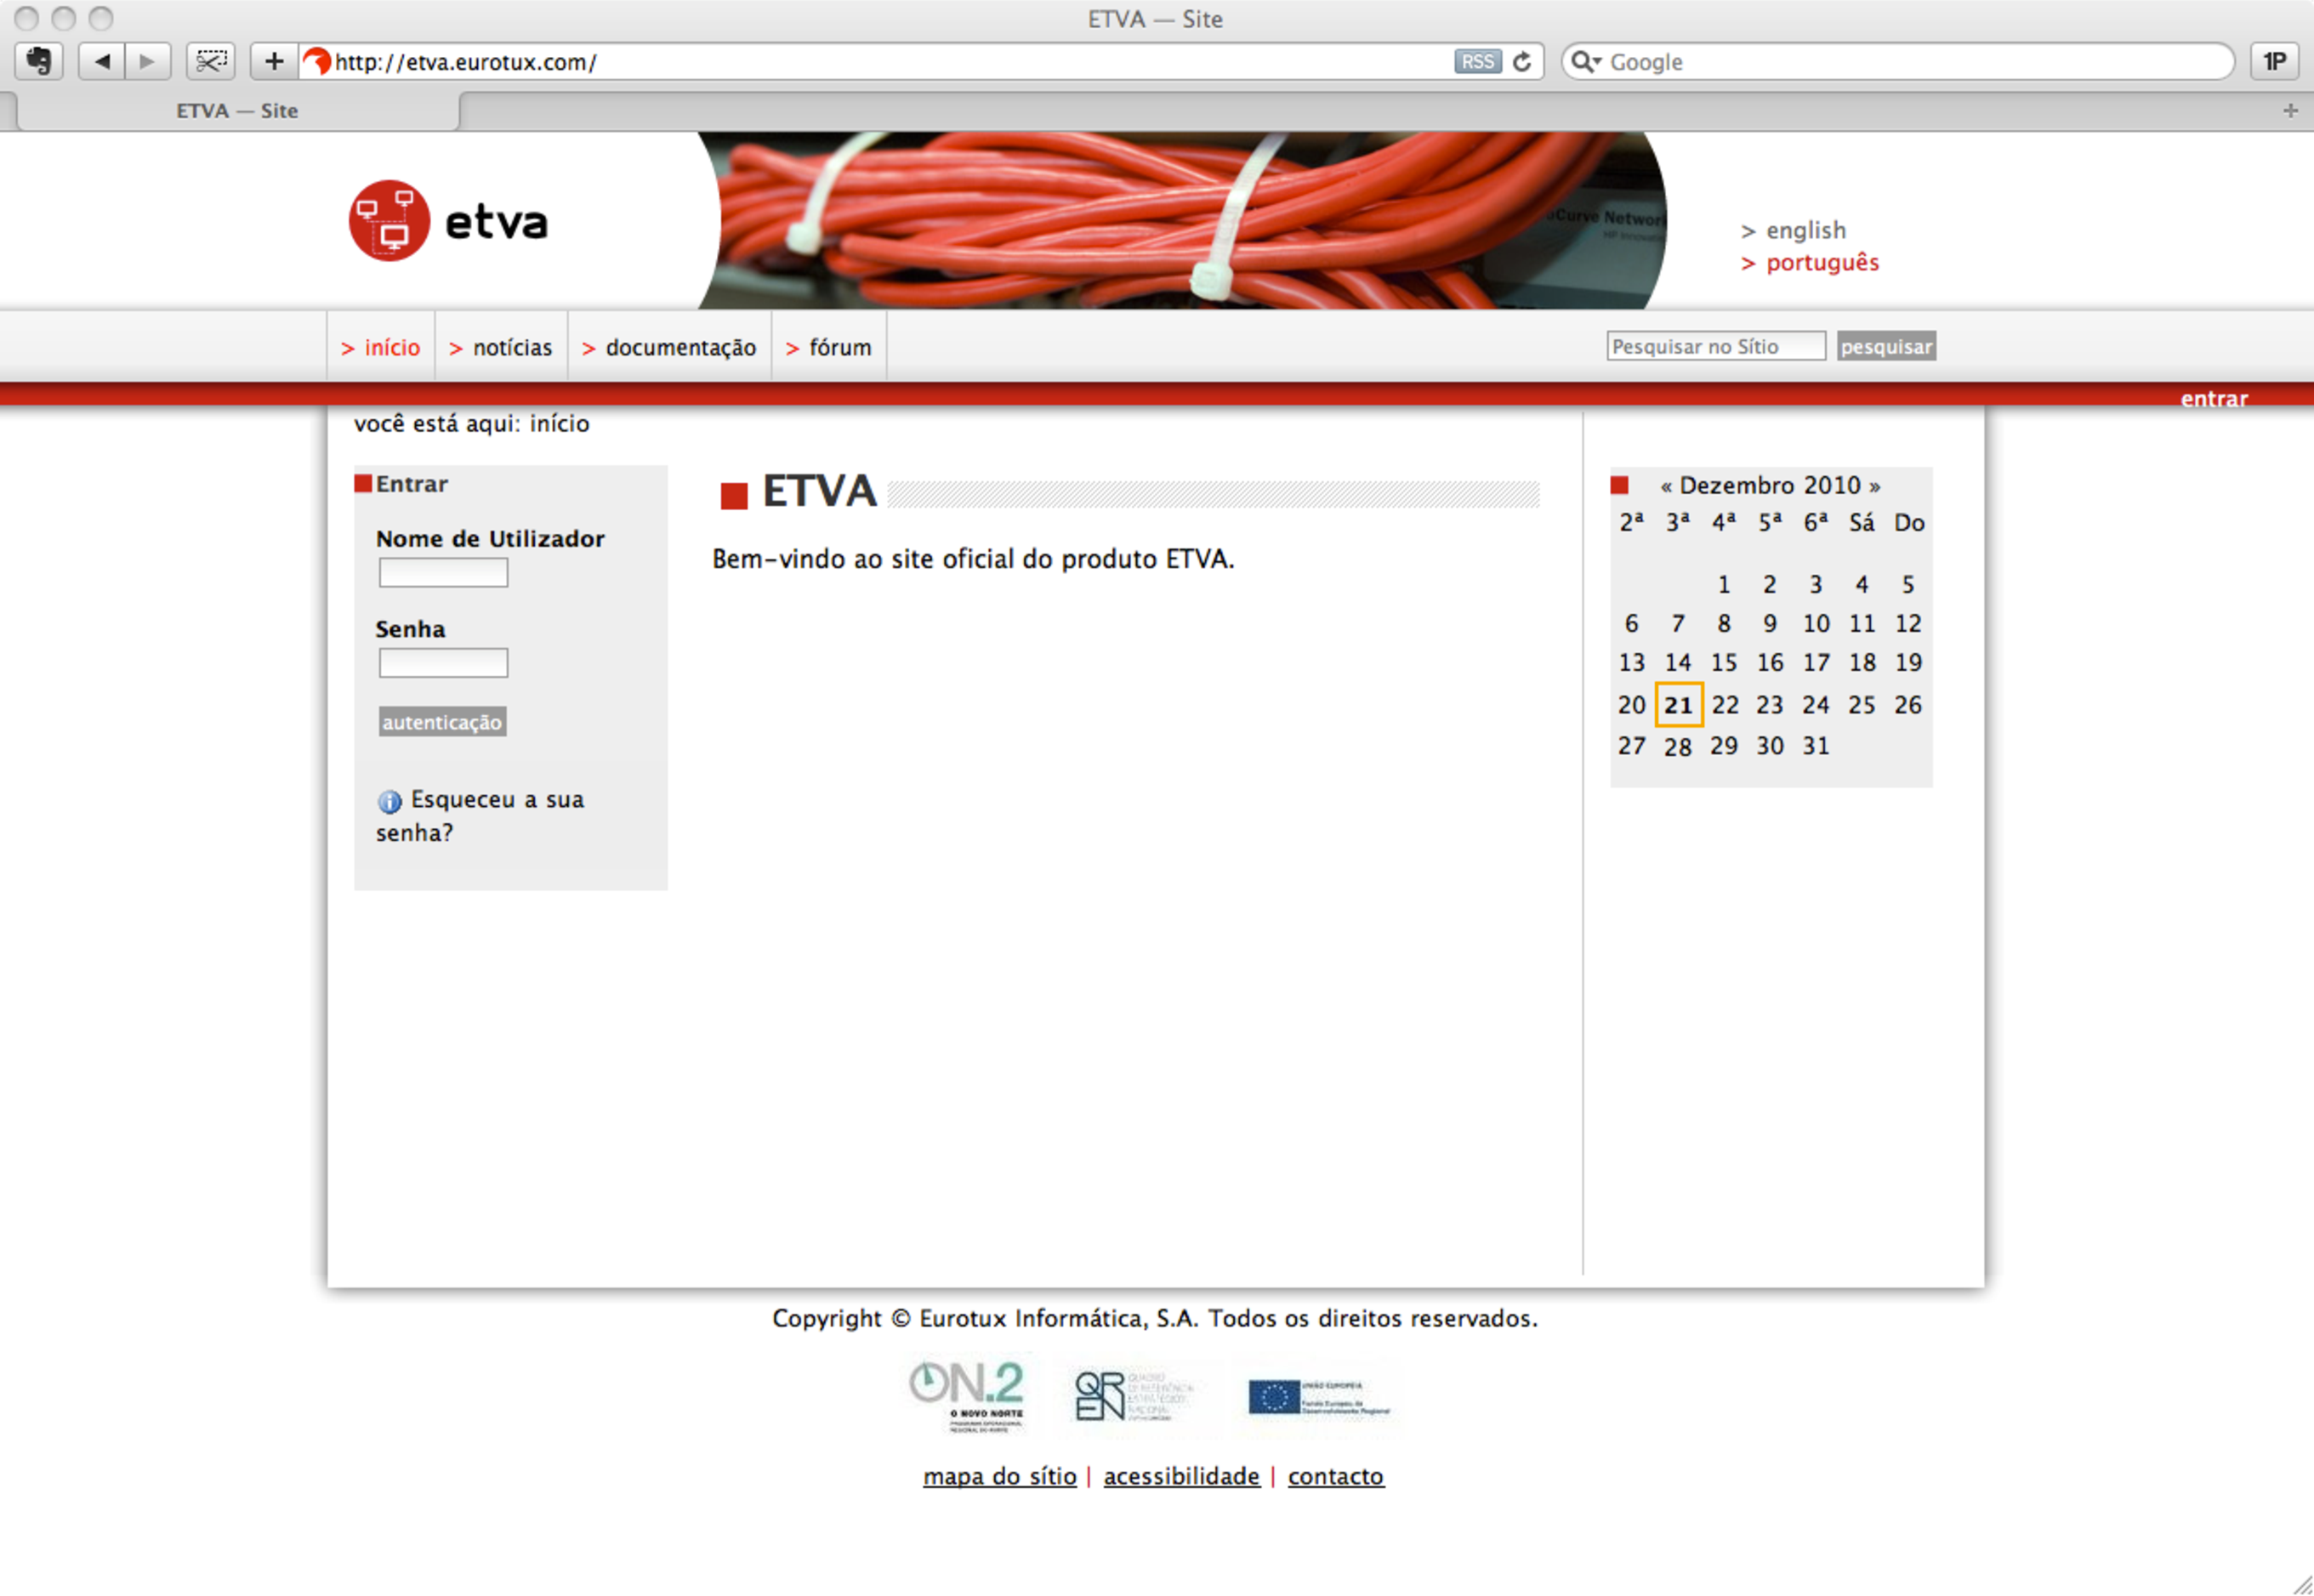
\includegraphics[scale=.35]{site}
	\caption{Página inicial do sítio web da ETVA.}
	\label{fig:logo}
\end{figure}


\paragraph{Desenvolvimento do sítio web do produto}

O site web do produto foi projectado e implementado, estando neste momento a
ser efectuada uma revisão do mesmo com vista ao lançamento do produto e com a
introdução de novos conteúdos.

\paragraph{Acções de marketing e divulgação}

Relativamente a esta tarefa ela está relativamente atrasada uma vez que
estamos à espera de ter datas previstas para a comercialização do produto
antes de inciarmos estas actividades.

A Eurotux criou num repositório de acesso livre, o github (http://github.com) um repositório com os desenvolvimentos do software associados ao ETVA (https://github.com/eurotux/ETVA)

\paragraph{Desenvolvimento de aplicações e infraestruturas de suporte ao canal
de comercialização e distribuição}

Em relação a esta tarefa, a Eurotux está activamente a procurar parceiros com
canal de distribuição já estabelecido de forma a agilizar a entrada do produto
no mercado. A Eurotux não tem ainda estabelecido um canal de distribuição,
pelo que acredita que esta será a forma mais eficiente de conseguir colocar o
produto no mercado, permitindo avançar em paralelo com a construção de um canal
de distribuição.

\subsubsection{Actividade 6 – Controlo de qualidade e certificação dos
processos associados à Eurotux Virtual Appliance}

Sendo este o primeiro grande projecto de investigação e desenvolvimento
liderado pela Eurotux, não estão ainda definidos os processos de gestão e
acompanhamento associados a este tipo de projectos. Esta actividade é de
especial importância, não só para este projecto mas também para projectos
futuros ao definir os métodos, métricas e processos a utilizar neste tipo de
projectos.

\paragraph{Definição de métricas, medidas, processos,  métodos e testes para verificação da qualidade dos produtos desenvolvidos}

Esta actividade decorreu como previsto e definiu uma nova metodologia a
utilizar pela Eurotux na execução de projectos de alguma dimensão, quer sejam
projectos de investigação, quer de desenvolvimento. Como resultado deste
projecto foi criado um repositório baseado em trac~\cite{trac} para gestão e
acompanhamento de projectos.


\paragraph{Preparação do processo de certificação dos processos de desenvolvimento e do produto}

Resultado das metodologias e processos definidos nesta actividade a Eurotux
decidiu implementar um sistema de qualidade de IDI segundo a norma NP 4457,
sendo que este projecto será um dos projectos a utilizar como referência.


\subsubsection{Actividade 7 – Gestão e acompanhamento do projecto}

Esta actividade que define uma tarefa de "Acompanhamento da evolução das
actividades e gestão do projecto" e que teve como principal objetivo garantir
a execução do projecto como previsto e caso fosse necessário sinalizaria, tal
como aconteceu as dificuldades e atrasos na execução do projecto.


% section resultados_obtidos (end)

\section{Deliverables e milestones} % (fold)
\label{sec:section_name}

Faz-se em seguida a enumeração dos milestones já concluídos por actividade e tarefa.

\subsection*{Actividade 1 - Arquitectura de Serviços da Eurotux Virtual Appliance} % (fold)
\label{sub:actividade_1}

\paragraph{Tarefa 1: Estado da arte em SOA (Service Oriented Architectures) para a gestão de infraestruturas computacionais} % (fold)

\subparagraph{Milestone1.1: Levantamento dos webservices e SOA relacionados com a administração de sitemas} % (fold)

\subparagraph{Milestone1.2: Caracterização dos webservices e SOA existentes} % (fold)


\paragraph{Tarefa 2: Definição dos Serviços a utilizar na Eurotux Virtual Appliance e no serviço de directoria} % (fold)


\subparagraph{Milestone 1.3: Proposta preliminar de SOA e webservices a utilizar na ETVA} % (fold)


\subparagraph{Milestone 1.4: Proposta preliminar de SOA e webservices a utilizar no Serviço de Directoria} % (fold)


\subparagraph{Milestone 1.5: Proposta de SOA e webservices a utilizar na ETVA} % (fold)



\paragraph{Tarefa 3: Implementação da arquitectura SOA e serviços na Eurotux Virtual Appliance} % (fold)
\label{par:implementação_da_arquitectura_soa_e_servios_na_eurotux_virtual_appliance}

\subparagraph{Milestone 1.6: Release alfa de SOA e webservices a utilizar na ETVA} % (fold)

\subparagraph{Milestone 1.7: Release beta de SOA e webservices a utilizar na ETVA} % (fold)

\subparagraph{Milestone 1.8: Release de SOA e webservices a utilizar na ETVA} % (fold)


\paragraph{Tarefa 4: Implementação do serviço de directoria} % (fold)
\label{par:implementação_do_serviço_de_directoria}


\subparagraph{Milestone 1.9: Release beta de  SOA e webservices a utilizar no Serviço de Directoria} % (fold)

\subparagraph{Milestone 1.10: Disponibilização do Serviço de Directoria} % (fold)


\subsubsection*{Actividade 2 – Desenvolvimento da Interface de Gestão da Eurotux Virtual Appliance} % (fold)


\paragraph{Tarefa 1: Concepção Gráfica} % (fold)

\subparagraph{Milestone 2.1: Proposta de design gráfico} % (fold)

\subparagraph{Milestone 2.2: Implementação do design gráfico} % (fold)


\paragraph{Tarefa 2: Concepção e Implementação da Interface de Gestão} % (fold)

\subparagraph{Milestone 2.3: Definição dos requisitos das interfaces dos produtos e aplicações} % (fold)

\subparagraph{Milestone 2.4: Disponibilização de uma versão alfa da interface} % (fold)


\subparagraph{Milestone 2.5: Disponibilização de uma versão beta da interface} % (fold)


%\subparagraph{Milestone 2.6: Disponibilização da versão final da interface} % (fold)

\subsubsection*{Actividade 3 – Migração dos produtos Eurotux para a Eurotux Virtual Appliance} % (fold)


\paragraph{Tarefa 1: Eurotux Virtual Firewall} 

\subparagraph{Milestone 3.1: Versão preliminar da Eurotux Virtual Firewall para a ETVA}


%\subparagraph{Milestone 3.2: Versão de produção da Eurotux Virtual Firewall para a ETVA}


\paragraph{Tarefa 2: Eurotux Virtual Mailserver}

\subparagraph{Milestone 3.3: Versão preliminar do Eurotux Virtual Mailserver para a ETVA}

%\subparagraph{Milestone 3.4: Versão de produção do Eurotux Virtual Mailserver para a ETVA}

\paragraph{Tarefa 3: Eurotux Virtual HotSpot}

\subparagraph{Milestone 3.5: Versão preliminar do Eurotux Virtual HotSpot para a ETVA}

\subparagraph{Milestone 3.6: Versão de produção do Eurotux Virtual HotSpot para a ETVA}


\paragraph{Tarefa 4: Eurotux Virtual VOIP server}

%\subparagraph{Milestone 3.7: Versão de produção do Eurotux Virtual VOIP server para a ETVA}

\subsubsection*{Actividade 4 – Avaliação e selecção das plataformas de hardware de suporte à Eurotux Virtual Appliance}

\paragraph{Tarefa 1: Definição dos requisitos de hardware para a Eurotux Virtual Appliance}

\subparagraph{Milestone 4.1: Definição dos requisitos de hardware da Eurotux Virtual Appliance}


\paragraph{Tarefa 2: Selecção das plataformas de hardware de suporte à Eurotux Virtual Appliance}

\subparagraph{Milestone 4.2: Seleccção das plataformas de suporte à Eurotux Virtual Appliance}

\subparagraph{Milestone 4.3: Reavaliação das plataformas de suporte à Eurotux Virtual Appliance}


\subsubsection*{Actividade 5 – Actividades de promoção e divulgação associadas à Eurotux Virtual Appliance}


\paragraph{Tarefa 1: Concepção e definição da imagem do produto}

\subparagraph{Milestone 5.1: Definição da imagem do produto}


\paragraph{Tarefa 2: Desenvolvimento do sítio web do produto}

\subparagraph{Milestone 5.2: Versão preliminar do sítio web do produto}

%\subparagraph{Milestone 5.3: Apresentação do sítio web do produto}

\paragraph{Tarefa 3: Acções de marketing e divulgação}

\paragraph{Tarefa 4: Desenvolvimento de aplicações e infraestruturas de suporte ao canal de comercialização e distribuição}

\subparagraph{Milestone 5.4: Apresentação da infraestrutura de suporte ao canal de distribuição}


\subsubsection*{Actividade 6 – Controlo de qualidade e certificação dos processos associados à Eurotux Virtual Appliance}

\paragraph{Tarefa 1: Definição de métricas, medidas, processos,  métodos e testes para verificação da qualidade dos produtos desenvolvidos}

\subparagraph{Milestone 6.1: Definição preliminar das metodologias e métodos para controlo da qualidade}

\subparagraph{Milestone 6.2: Dproposta de metodologias processos para controlo da qualidade}


\paragraph{Tarefa 2: Preparação do processo de certificação dos processos de desenvolvimento e do produto}

\subparagraph{Milestone 6.3: Dossiers para os processos de certificação}


\subsubsection*{Actividade 7 – Gestão e acompanhamento do projecto}

\paragraph{Tarefa 1: Acompanhamento da evolução das actividades e gestão do projecto}

\subparagraph{Milestone 7.1: Progresso e evolução do projecto (6 meses)}

\subparagraph{Milestone 7.2: Progresso e evolução do projecto (12 meses)}

\subparagraph{Milestone 7.3: Progresso e evolução do projecto (28 meses)}

\subparagraph{Milestone 7.4: Progresso e evolução do projecto (24 meses)}

%\subparagraph{Milestone 7.5: Conclusão do projecto}




%  4- Identificação dos Deliverables e
% Milestones Liste os deliverables e os milestones identificados para período do
% relatório, conforme indicado na candidatura.
% section section_name (end)

% \section{Actividades de valorização} % (fold)
% \label{sec:actividades_de_valorização}

% section actividades_de_valorização (end)


\section{Fotografias} % (fold)
\label{sec:fotografias}

Apresentam-se de seguida fotografias das infraestruturas utilizadas no projecto, nomeadamente a appliance para o mercado de pequenas e médias empresas (Figura~\ref{fig:smb}) e do modelo enterprise que suportou todo o desenvolvimento do produto (Figura~\ref{fig:blades}).

\begin{figure}[htbp]
	\centering
		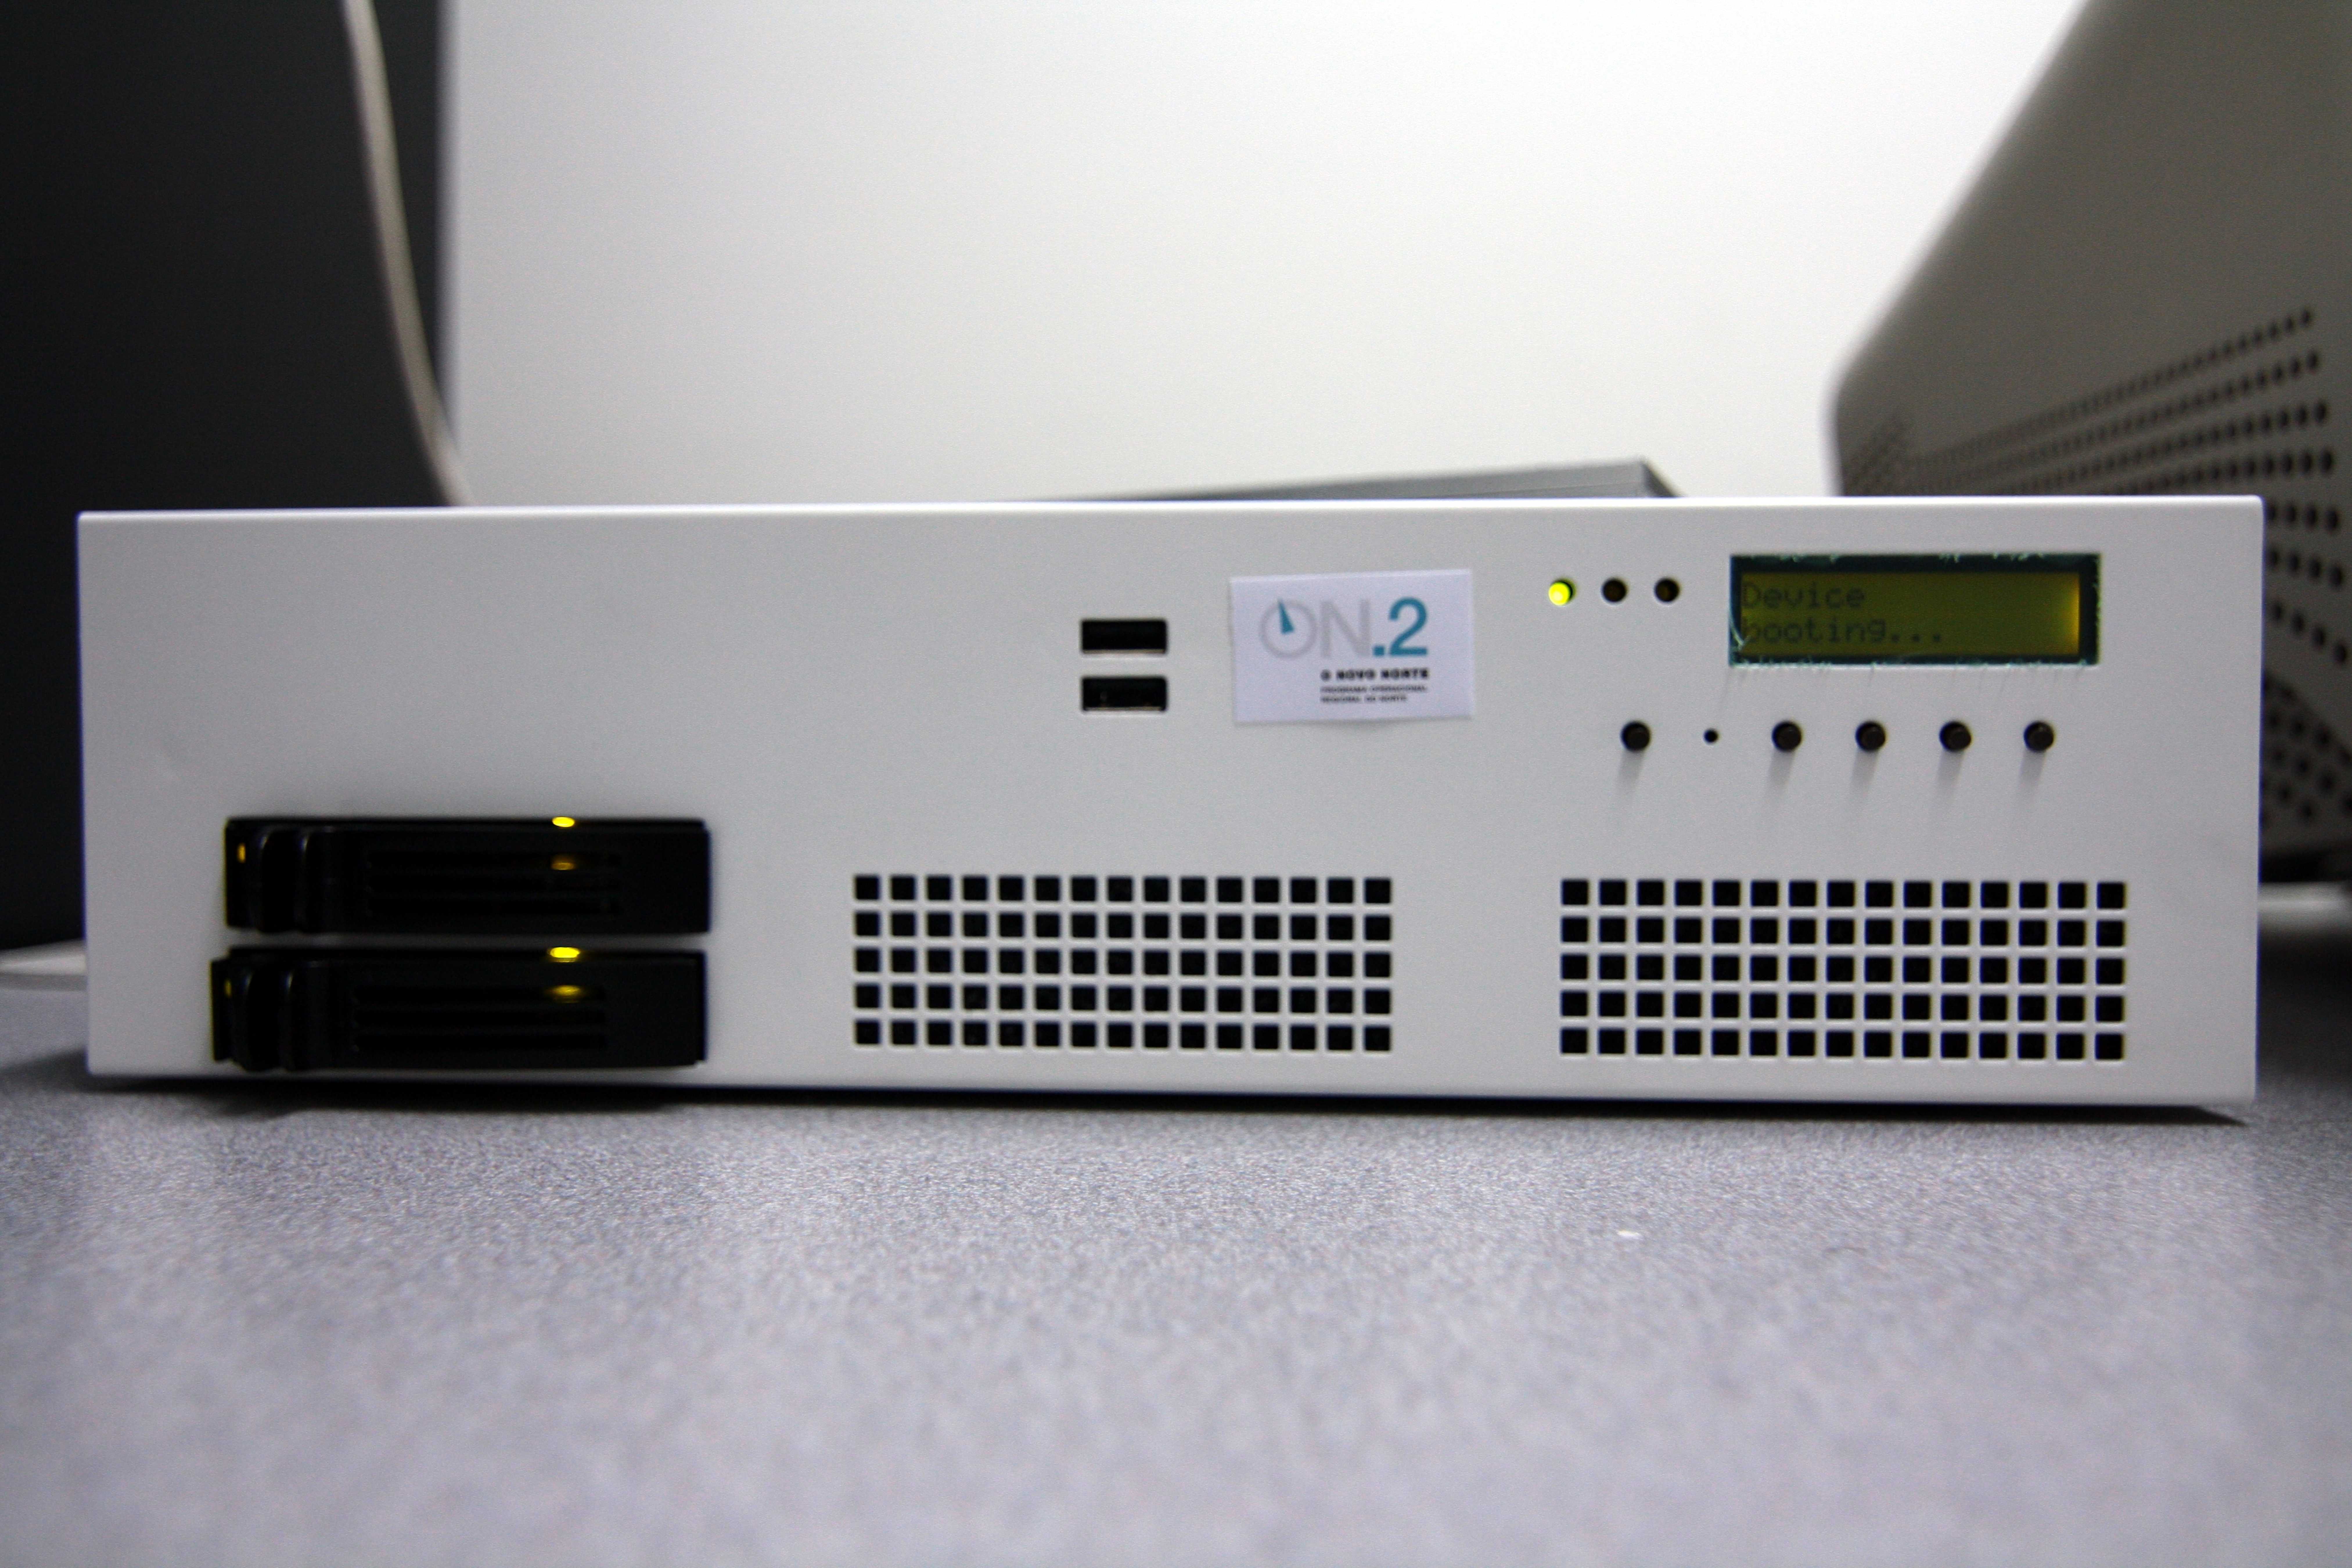
\includegraphics[width=.5\textwidth]{smb}
	\caption{Appliance ETVA para smb.}
	\label{fig:smb}
\end{figure}


\begin{figure}[h!]
	\centering
		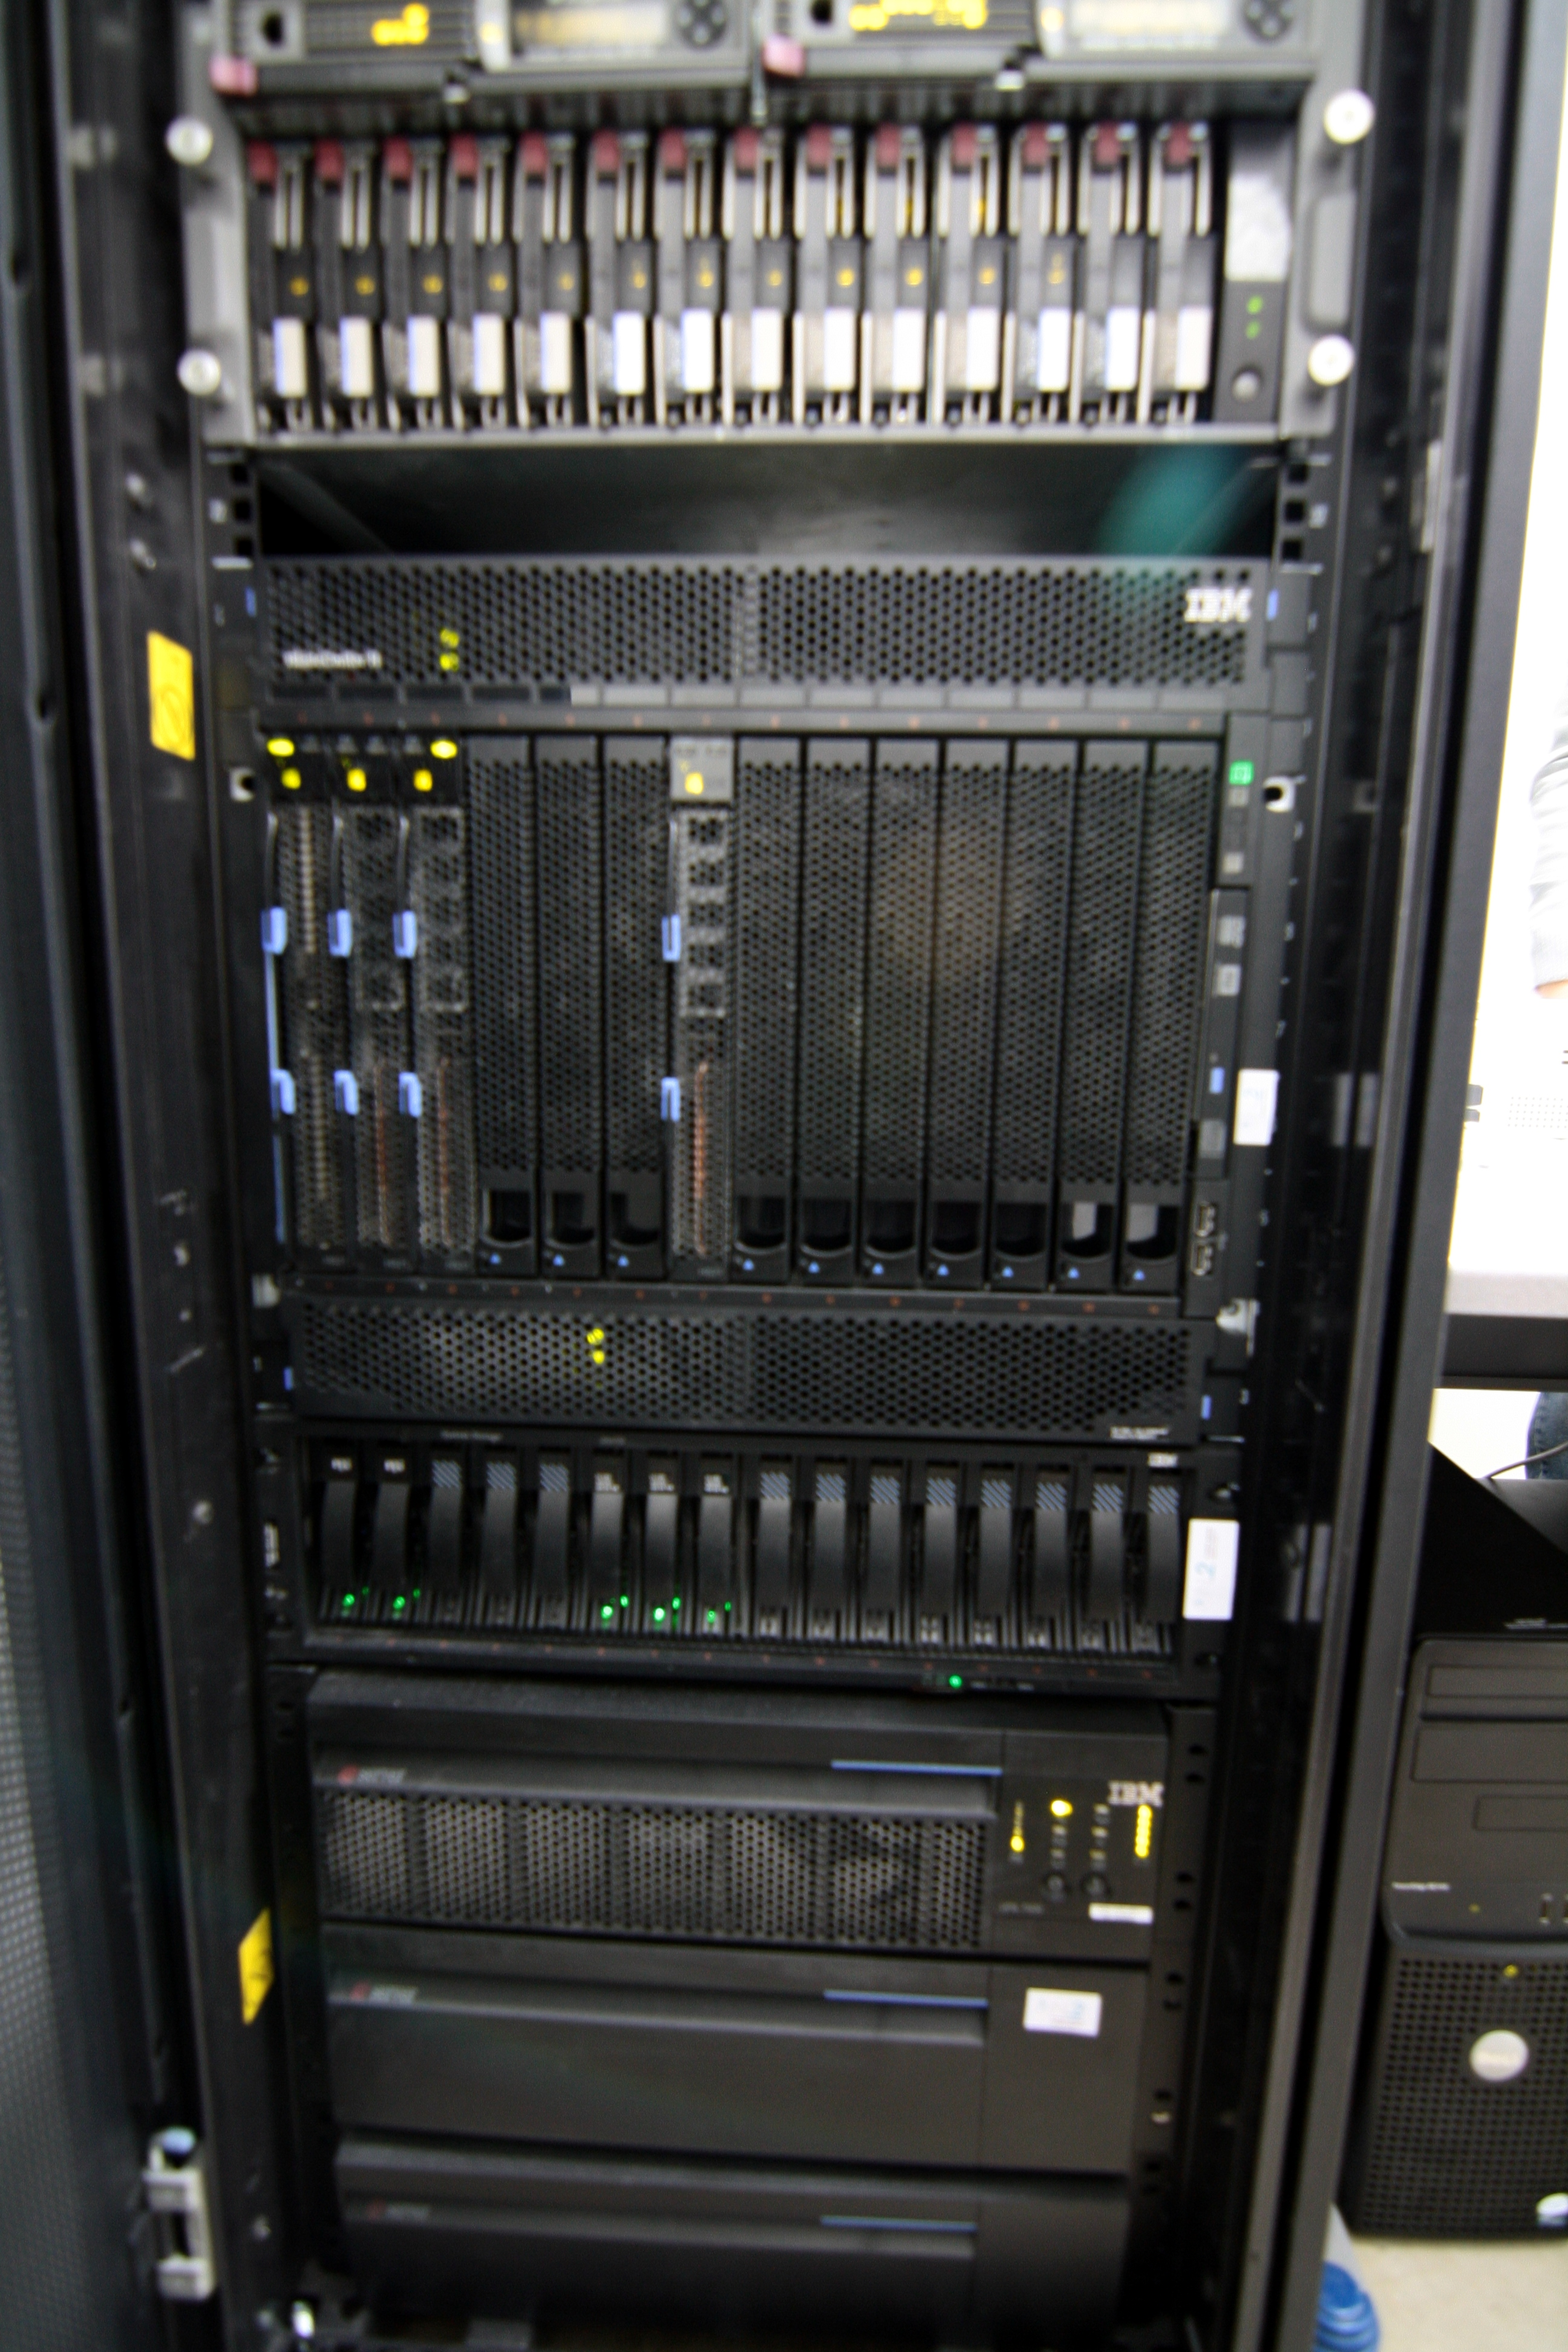
\includegraphics[width=.4\textwidth]{blades}
	\caption{Infraestrutura ETVA modelo enterprise.}
	\label{fig:blades}
\end{figure}
%\newpage
% section fotografias (end)
\bibliographystyle{plain}
\bibliography{relatorio-tec-cientifico}
\end{document}

Boa tarde, Drª Cristina Vasconcelos

Dado que no âmbito dos projectos de I&DT, a verificação da execução material
do projecto é suportada por relatórios técnico-científicos, em português, que
têm como objectivo demonstrar a evolução do projecto ao nível da sua execução
física, deverão V. Exas proceder ao envio do documento referido, o qual deverá
ser elaborado de acordo com a seguinte estrutura:

1- Sumário executivo das actividades do projecto e dos resultados alcançados
Nesta secção inclua uma descrição sucinta dos objectivos do projecto, do
trabalho realizado desde o início do projecto e dos principais resultados
alcançados até ao período de reporte.

2- Diagrama de Gantt comparando o trabalho previsto na candidatura com o
realizado 

3- Apresentação dos resultados alcançados por tarefa, justificando
eventuais desvios face ao previsto em candidatura Se aplicável, explicite
alterações aos objectivos críticos definidos, por não terem sido atingidos
e/ou por os desenvolvimentos terem gerado novos resultados intermédios,
justificando o impacto no projecto.

 4- Identificação dos Deliverables e
Milestones Liste os deliverables e os milestones identificados para período do
relatório, conforme indicado na candidatura. 
5- Apresentação das actividades
de valorização dos resultados realizadas (divulgação, patentes, …), se
aplicável 
6- Fotografias (se aplicável)

Os relatórios intercalares devem ser apresentados sempre que seja efectuado um
pedido de pagamento ou com a periodicidade não superior a 12 meses.

Com os melhores cumprimentos Normando Faria

IAPMEI - Instituto de Apoio às Pequenas e Médias Empresas e à Inovação DGIC -
Direcção de Gestão de Incentivos e de Créditos DpVS Norte – Departamento de
Acompanhamento e Verificação para os Serviços e Outros Sectores Rua de
Salazares, 842 – 4100 -442 PORTO Telefone: 226 152 034| Fax: 226 152 022
